%%%%%%%%%%%%%%%%%%%%%%%%%%%%%%%%%%%%%%%%%
%
% (c) 2019 by Jennifer Laaser
%
% This work is licensed under the Creative Commons Attribution-NonCommercial-ShareAlike 4.0 International License. To view a copy of this license, visit http://creativecommons.org/licenses/by-nc-sa/4.0/ or send a letter to Creative Commons, PO Box 1866, Mountain View, CA 94042, USA.
%
% The current source for these materials is accessible on Github: https://github.com/jlaaser/pogil-polymers
%
%%%%%%%%%%%%%%%%%%%%%%%%%%%%%%%%%%%%%%%%%

\renewcommand{\figpath}{content/polymphys/mechanical-properties/SAOS/figs}
\newcommand{\labelbase}{}
\renewcommand{\labelbase}{viscoelasticity}

\begin{activity}[Small-Amplitude Oscillatory Shear Rheology]

\begin{instructornotes}

	This activity introduces students to important concepts in small-amplitude oscillatory shear rheology.
	
	After completing this activity, students will be able to:
			\begin{enumerate}
				\item Explain what a small-amplitude oscillatory shear rheology experiment is
				\item Explain what the ``storage modulus'' and ``loss modulus'' of a material are
				\item Interpret data from a small-amplitude oscillatory shear rheology experiment in terms of the liquid- or solid-like properties of the material and the characteristic relaxation time
			\end{enumerate}
	
			
	\subsection*{Activity summary:}
	\begin{itemize}
		\item \textbf{Activity type:} Learning Cycle
		\item \textbf{Content goals:} Explaining SAOS experiments
		\item \textbf{Process goals:} %https://pogil.org/uploads/attachments/cj54b5yts006cklx4hh758htf-process-skills-official-pogil-list-2015-original.pdf
			\begin{itemize}
				\item Interpreting equations in terms of physical behavior
				\item Reading and interpreting graphs
			\end{itemize}
		\item \textbf{Duration:} approx. 30 min
		\item \textbf{Instructor preparation required:} 
			\begin{itemize}
				\item n/a
			\end{itemize}
		\item \textbf{Related textbook chapters:}
			\begin{itemize}
				\item \emph{Polymer Chemistry} (Hiemenz \& Lodge): Sections 11.2.4 and 11.8
			\end{itemize}
	\end{itemize}

\end{instructornotes}

	%\textbf{Focus question:} Put a central question for the students to consider through this exercise here.


\begin{model}[Small-Amplitude Oscillatory Shear Rheology]
\label{model:rheology}

	One of the most common experimental techniques used to characterize the viscoelasticity of polymeric materials is small-amplitude oscillatory shear rheology (SAOS).
	
	In a SAOS measurement, the sample is sandwiched between two surfaces that rotate back and forth at frequency $\omega$, resulting in a sinusoidally-varying strain:
	\begin{equation*}
		\gamma(t) = \gamma_0 \sin(\omega t)
	\end{equation*}
	
	The instrument (a rheometer) then measures the resulting force as a function of time, $\sigma(t)$, and breaks it down into two components: one that is proportional to $\sin(\omega t)$ and one that is proportional to $\cos(\omega t)$. The response of the material can thus be expressed as follows:
	\begin{equation*}
		G(t) = \frac{\sigma(t)}{\gamma_0} = G' \sin(\omega t) + G'' \cos(\omega t)
	\end{equation*}

\end{model}

%\vspace{0.25in}
\begin{ctqs}
		
		\question In this experiment, the strain is proportional to $\sin(\omega t)$.  
			\begin{enumerate}
				\item Which coefficient, $G'$ or $G''$, tells you how much of the response is directly proportional to the applied strain?
	
					\begin{solution}[1in]
						$G'$ is in the term that goes as $\sin(\omega t)$, so $G'$ is the coefficient that tells us how much of the response is directly proportional to the applied strain.
					\end{solution}
		
		\item Does this coefficient tell you about the elastic response of the material, or the viscous response of the material?
	
					\begin{solution}[1in]
						The elastic response is directly proportional to the applied strain, so this coefficient tells us about the elastic response.
					\end{solution}
					
			\end{enumerate}
			
		\question Since $\frac{d}{dt}\sin(\omega t) \sim \cos(\omega t)$, the strain \emph{rate} in this experiment is proportional to $\cos(\omega t)$.
		
			\begin{enumerate}
		
				\item Which coefficient, $G'$ or $G''$, tells you how much of the response is proportional to the strain rate?
	
					\begin{solution}[1in]
						The $G''$ term is proportional to $\cos(\omega t)$, so $G''$ tells us about the portion of the response that is proportional to strain rate.
					\end{solution}
		
				\item Does this coefficient tell you about the elastic response of the material, or the viscous response of the material?
	
					\begin{solution}[1in]
					
						The viscous response is proportional to the strain rate, so this coefficient tells us about the viscous repsonse.
					
					\end{solution}
					
			\end{enumerate}
		
		\question Remembering that elastic responses store energy, and viscous responses dissipate energy, explain why we call $G'$ the ``storage modulus'' and $G''$ the ``loss modulus'' of the material.
	
					\begin{solution}[2in]
					
						$G'$ gives information about the elastic response, which stores energy, so $G'$ is called the storage modulus.
						
						$G''$ gives information about the viscous response, which dissipates energy, so $G''$ is called the loss modulus.
					\end{solution}
			
\end{ctqs}

\clearpage
\begin{model}
	As shown in Exercise \ref{\labelbase:exc:Boltzmann}, the storage and loss moduli for the Maxwell Model are given by:
	\begin{align*}
		G' = G_0 \frac{\omega^2 \tau^2}{\omega^2 \tau^2 + 1} && \text{and} && G'' = G_0 \frac{\omega \tau}{\omega^2 \tau^2 + 1}
	\end{align*}
	
	A plot of these moduli as a function of frequency is given below:
			
		\vspace{0.1in}	
		\centerline{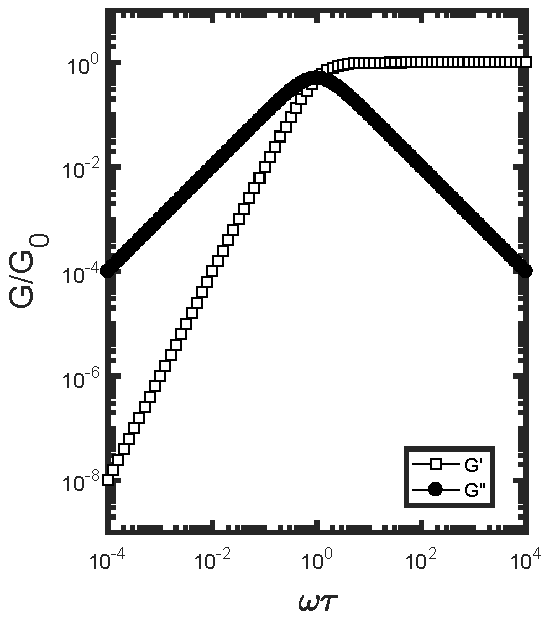
\includegraphics[width=0.4\textwidth]{\figpath/model1-maxwellplot}}
	
	Note that both axes of this graph are plotted on a log scale; the x axis has been scaled by the characteristic relaxation time, $\tau$, and the y axis has been scaled by the modulus, $G_0$.
	
\end{model}

\begin{ctqs}
	
	\question First, consider the low-frequency portion of the response:
	
		\begin{enumerate}
		
			\item  At low frequencies, which is larger, the storage modulus or the loss modulus?
	
					\begin{solution}[0.5in]
					
						According to the plot, the loss modulus is larger at low frequencies.
					
					\end{solution}
					
			\item Do low frequency measurements correspond to fast (short) timescales, or long (slow) timescales?
	
		\end{enumerate}
	
	\question Now, consider the high-frequency portion of the response:
	
		\begin{enumerate}
		
			\item At high frequencies, which is larger, the storage modulus or the loss modulus?
	
					\begin{solution}[0.5in]
					
						According to the plot, the storage modulus is larger at high frequencies.
					
					\end{solution}
		
			\item At high frequencies (corresponding to short observation timescales), which is greater, the storage modulus or the loss modulus?  Is this consistent with your expectations?  Briefly explain your answer in 1-2 complete sentences.
	
					\begin{solution}[1.1in]
					
						At high frequencies, the storage modulus is greater.  This makes sense, because on long timescales, the material should be mostly solid-like.
					\end{solution}
	\end{enumerate}

	\question At what frequency is the storage modulus exactly equal to the loss modulus?  Give your answer in terms of the characteristic relaxation time, $\tau$.
	
		\emph{Note: you can answer this using either the graph or the equations, but you will probably find it easier to work from the equations.}
	
					\begin{solution}[1.75in]
					
						Setting the equations for $G'$ and $G''$ equal to each other, we have
						\begin{align*}
							G' &= G''\\
							G_0 \frac{\omega^2 \tau^2}{\omega^2 \tau^2 + 1} &= G_0 \frac{\omega \tau}{\omega^2 \tau^2 + 1}\\
							\omega^2 \tau^2 &= \omega \tau\\
							\omega\tau &= 1\\
							\omega &= \frac{1}{\tau}
						\end{align*}
					\end{solution}
	
	\question Rearrange your answer to the previous question to find an expression for the characteristic relaxation time in terms of the crossover frequency.
	
					\begin{solution}[1in]
					
						\begin{align*}
							\tau = \frac{1}{\omega_c}
						\end{align*}
					\end{solution}
	
\end{ctqs}
	

%\clearpage
\begin{exercises}

		\exercise \label{\labelbase:exc:Boltzmann} DERIVE RESPONSE FOR SAOS USING BOLTZMANN?

		\exercise Consider the polymer characterized in the following plot:
				
		\centerline{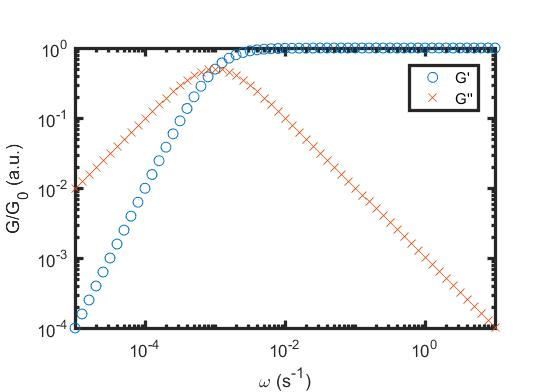
\includegraphics[width=0.6\textwidth]{\figpath/model2-maxwellexample.jpg}}
		
		\begin{enumerate}
		
			\item Find the characteristic relaxation time of this polymer.
	
					\begin{solution}
					
						The storage and loss moduli are equal when $\omega=10^{-3}\text{ s}^{-1}$.  Thus the characteristic relaxation time is
						
						\begin{equation*}
							\tau = \frac{1}{\omega_c} = \frac{1}{10^{-3}\text{ s}^{-1}} = 1000\text{ s} \approx 17\text{ min}
						\end{equation*}
					\end{solution}
	
			\item If you were to pick up a sample of this polymer, would you expect it to feel more like a liquid or more like a solid?  Briefly justify your answer.
	
			\emph{Hint: think about how the timescale on which you are observing/interacting with the polymer compares to the relaxation time!}
	
					\begin{solution}
					
						This polymer would probably feel more like a solid.  When we pick a material up, we are typically observing it on timescales on the order of a second.  This timescale is much shorter than the characteristic relaxation time of the material, so we will observe primarily solid-like properties.
					
					\end{solution}
					
		\end{enumerate}
		
\end{exercises}
	
\end{activity}